\documentclass[border=4pt]{standalone}
% Shared typography and colours for the standalone figures.
\usepackage{unicode-math}
\setmainfont{TeX Gyre Termes}
\setsansfont{TeX Gyre Heros}
\setmonofont{TeX Gyre Cursor}
\setmathfont{TeX Gyre Termes Math}
\usepackage{tikz}
\usetikzlibrary{arrows.meta,positioning,calc,decorations.pathreplacing}
\usepackage{pgfplots}
\pgfplotsset{compat=1.18}
\definecolor{elemA}{HTML}{1F5FA8}
\definecolor{elemB}{HTML}{B8461B}
\definecolor{elemC}{HTML}{2E7D32}
\definecolor{elemD}{HTML}{6A4C93}
\definecolor{frameline}{HTML}{555555}

\begin{document}
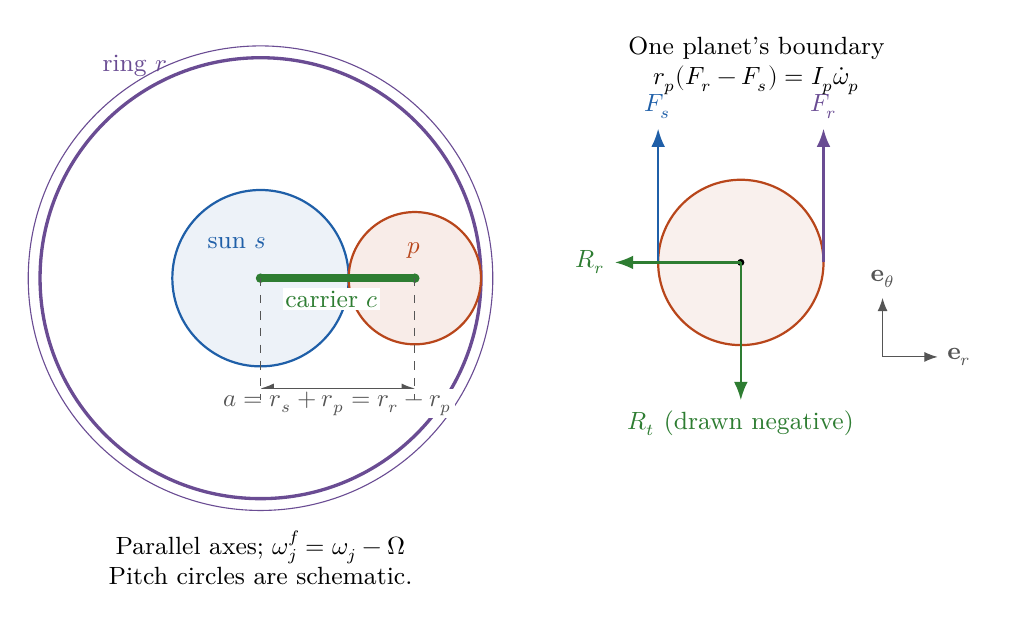
\begin{tikzpicture}[>=Latex,font=\small]
\draw[elemD,very thick] (0,0) circle (2.8);
\draw[elemD] (0,0) circle (2.95);
\draw[elemA,thick,fill=elemA!8] (0,0) circle (1.12);
\draw[elemB,thick,fill=elemB!10] (1.96,0) circle (.84);
\draw[elemC,line width=3pt] (0,0)--(1.96,0);
\fill[elemC] (0,0) circle (.06) (1.96,0) circle (.06);
\node[elemA] at (-.3,.45) {sun $s$};
\node[elemB] at (1.95,.35) {$p$};
\node[elemC,below,fill=white,inner sep=1pt] at (.9,-.12) {carrier $c$};
\node[elemD] at (-1.6,2.7) {ring $r$};
\draw[<->,frameline] (0,-1.4)--node[below,fill=white,inner sep=1pt] {$a=r_s+r_p=r_r-r_p$}(1.96,-1.4);
\draw[dashed,frameline] (0,0)--(0,-1.55) (1.96,0)--(1.96,-1.55);
\node[align=center] at (0,-3.55) {Parallel axes; $\omega_j^f=\omega_j-\Omega$\\Pitch circles are schematic.};
\begin{scope}[xshift=6.1cm,yshift=.2cm]
\draw[elemB,thick,fill=elemB!8] (0,0) circle (1.05);
\fill (0,0) circle (.045);
\draw[->,thick,elemA] (-1.05,0)--(-1.05,1.7) node[above] {$F_s$};
\draw[->,thick,elemD] (1.05,0)--(1.05,1.7) node[above] {$F_r$};
\draw[->,thick,elemC] (0,0)--(0,-1.75) node[below] {$R_t$ (drawn negative)};
\draw[->,thick,elemC] (0,0)--(-1.6,0) node[left] {$R_r$};
\draw[->,frameline] (1.8,-1.2)--(2.5,-1.2) node[right] {$\mathbf e_r$};
\draw[->,frameline] (1.8,-1.2)--(1.8,-.45) node[above] {$\mathbf e_\theta$};
\node[align=center] at (.2,2.5) {One planet's boundary\\$r_p(F_r-F_s)=I_p\dot\omega_p$};
\end{scope}
\end{tikzpicture}
\end{document}
